\subsubsection{The model}
The results are mainly the model that predicts the occurrence of a \ac{cs} or natural delivery. The evaluation metrics are present in the table below for the best hyper-parameters found for the training data.

\begin{table}[htbp]
  \centering
  \caption[Performance Metrics in the training set]{Performance Metrics in the training set with mean AUROC and 95\% Confidence Interval}
  \label{tab:performancemetricsauc}
  \renewcommand{\arraystretch}{1.5} % Adjust the vertical spacing
  \setlength{\tabcolsep}{12pt} % Adjust the horizontal spacing
  \begin{tabular}{lcc}
    \hline
    \textbf{Metric} & \textbf{AUROC} & \textbf{CI 95\%} \\
    \hline
    xgboost & 0.8809 & 0.8799, 0.882 \\  
    Decision Tree & 0.8337 & 0.8324, 0.8349 \\
    Logistic Regression & 0.8716 & 0.8706, 0.8726 \\
    AdaBoost & 0.8753 & 0.874, 0.8766 \\ 
    lightgbm & 0.8805 & 0.8793, 0.8817 \\ 
    Stochastic Gradient Descent & 0.8704 & 0.8694, 0.8713 \\ 
    Random Forest & 0.8752 & 0.8743, 0.8762 \\  
    \hline
  \end{tabular}
\end{table}

\ac{xgboost} and \ac{lightgbm} were the best-performing algorithms. However, we selected \ac{lightgbm} \cite{lightgbm} since it is faster and requires less memory. The threshold selected for deploying the model was 0.7457247885715557 which rendered the metrics in the test set like it is shown in table \ref{tab:performancemetricsthreshold}.

\begin{table}[htbp]
  \centering
\caption{Performance Metrics in the test set with chosen threshold}
\label{tab:performancemetricsthreshold}
\renewcommand{\arraystretch}{1.5} % Adjust the vertical spacing
\setlength{\tabcolsep}{12pt} % Adjust the horizontal spacing
\begin{tabular}{lc}
    \hline
    \textbf{Metric} & \textbf{Value} \\
    \hline
    Accuracy & 0.8052 \\
    Sensitivity & 0.8223 \\
    Precision & 0.9023 \\
    F1 Score & 0.8605 \\
    \hline
  \end{tabular}
\end{table}




\subsubsection{Deployment}
The purpose of this model is to be served as a \ac{api} for usage within a healthcare institution and act as a supplementary management decision support tool for obstetrics teams. And for that to happen, a health information system must make the requests to the API. Even though a concrete, vendor-specific information model and input health information system were used, we hope to create a more interoperable clinical decision support system which can be used by every system that acts upon births and obstetrics departments. That is why we built it around the \ac{hl7} \ac{fhir} standard (R5 version) in order to simplify the method of interacting with the API. This decision, opposed as to using a proprietary model for the data, sits upon the usage of \ac{fhir} resources: Bundle and Observation for request and returning the result as a message through a custom operation called "\$predict". It is intended to publish the profiles of these objects in order to facilitate access to the API using standardized mechanisms and data models - current build of the profiles \url{https://joofio.github.io/obs-cdss-fhir/}. The current spec is detailed in the following link. The process is identified in figure \ref{fig:deploy}.
We deployed this model in production in a single hospital and without a user interface, only collecting the data and prediction for later discussion and analysis. We collected 3231 requests. During this time, the number of alarms that were triggered was 123 (3.8\%). From this, we tried to understand the level of certainty for the decision and check the difference from the threshold of these alarms. The distance to the threshold for 73 was lower than 0.1 and was bigger than 0.1 for 50 (1.55\%) cases.

%TC:ignore

\begin{figure}[htbp]
\centering
\captionsetup{justification=centering}
\caption{Deployment and decision mechanism of the model}\label{fig:deploy} 
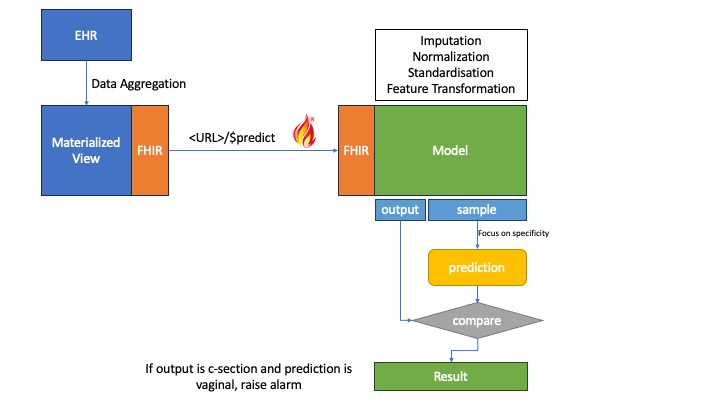
\includegraphics[scale=0.60]{figures/obs-model.jpg}
\end{figure}
%TC:endignore

\subsubsection{Clinical Evaluation}
The clinical evaluation was done by sending questionnaires to clinicians with a relationship with obstetrics in order to assess 10 patients, with only access to the variables used by the model and to answer 3 questions for each. The first was to give a score from 1-10 of how likely that patient would give birth through \ac{cs}, then to select the feature/variable that most influenced the decision and which feature they would require to make a better assessment. We sent the questionnaire to 20 people and got 6 answers. This rendered the results in figure \ref{fig:clinical}. We also predicted the result with the model as stated in figure \ref{fig:clinical}. These patients were new and not seen ever by the model in the training phase. 
As for the analysis of the most important features and missing features, the missing features were categorized into 3 categories: 1) Existent in the dataset but not included in the model, 2) Non-existent in the dataset and 3) existent in the dataset and included but that particular information was not filled for the patient assessed. This rendered a total of 62\% non-existent and 38\% existent but no information was provided at that moment. No feature mentioned existed but had not been included in the model. From the non-existent, 38\% were new clinical assessments, 38\% were linked to information from previous births,  15\% connected in more in-depth information about provided information (i.e, motive for induction) and 11\% were related to the mother's choice (if she wanted a \ac{cs}).
As for feature importance, from the 60 answers, we got 55\% with labour being the most important factor. 15\% answered the number of previous vaginal births, 8\% the evolution of weight and another 8\% the number of previous \acp{cs}. The remaining 14\% were various features, from \ac{bmi}, neuroaxis techniques, gestational age and weight of the mother. Of all of these, 90\% were included and were in the top 10 features of the model.



%TC:ignore

\begin{figure}[htbp]
\centering
\captionsetup{justification=centering}
\caption[Obstetrics questionnaires data]{Validation data. The colour represents the actual birth type. The boxplot represents the median and \ac{iqr} of the reviewers and the X represent each patient case. Contains 6 Vaginal births and 4 \acp{cs}. * represents wrong predictions of the model.}\label{fig:clinical} 
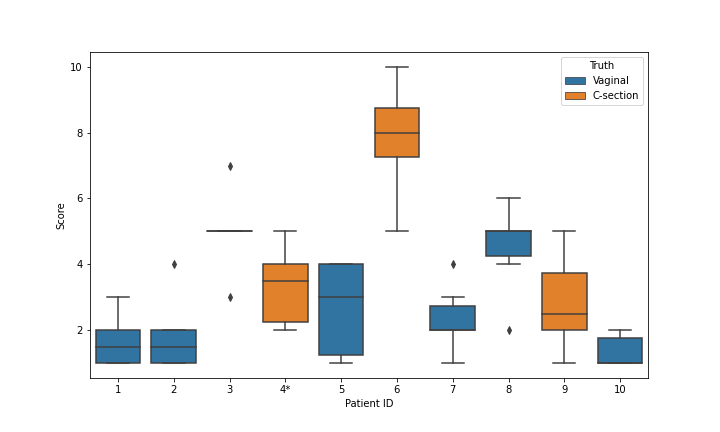
\includegraphics[scale=0.60]{figures/clinical_assessment.png}
\end{figure}
%TC:endignore




\subsubsection{Potential Financial Impact}
The financial support provided to public hospitals in Portugal is partially tied to the rate of \acp{cs}. To assess the potential impact of this mechanism on all Portuguese public hospitals, we conducted a simulation study. We got data for every public hospital for the last 12 months \cite{pordatacesarianas} and applied a reduction of 3.8\% (the rate of warnings triggered in the new dataset) and recalculated the rate of \acp{cs}. The increase in support was calculated by the state-mandated rate as shown in table \ref{tab:corrections}. With this new rate, we observed that implementing our tool would result in financial benefits for 30\% (11 hospitals) of the public hospitals. Specifically, five hospitals would begin receiving support instead of no support at all. Three hospitals would experience a doubling of their financial benefit, while two hospitals would see a 50\% increase. Furthermore, one hospital would receive an additional one-third of financial support.
If we assumed that only half of the warnings found in the new data were actually true (1.9\%) we found that only 6 hospitals would be benefited. 3 from 0 to 0.25, 2 from 0.25 to 0.50 and 1 from 0.50 to 0.75.


\begin{table}[htbp]
  \centering
  \caption[Ruleset for financial support indexed to \acsp{cs}.]{Ruleset for state-provided financial support indexed to \acp{cs}. X is the current payment of a \ac{cs} inpatient episode. Adapted from \cite{acssTermosReferenciaPara2023}}
  \label{tab:corrections}
  \renewcommand{\arraystretch}{1.2} % Adjust the vertical spacing
  \setlength{\tabcolsep}{12pt} % Adjust the horizontal spacing
  \begin{tabular}{lc}
      \hline
Rate of \acp{cs}   & Support \\
    \hline
\textless 25\%       & x       \\
{[}25\%, 26.4\%{]}   & 0.75 x   \\
{[}26.5\%, 27.9\%{]} & 0.5 x    \\
{[}28\%, 29.4\%{]}   & 0.25 x   \\
\textgreater{}29.5\% & 0      \\
    \hline
\end{tabular}
\end{table}